\documentclass[12pt]{article}
\usepackage{fontspec}
\usepackage{polyglossia}
\usepackage{amsmath}
\usepackage{amssymb}
\usepackage{xcolor}
\usepackage{fancyhdr}
\usepackage{graphicx}
\usepackage{listings}
\usepackage{geometry}

\pagestyle{fancy}

\setmainlanguage{arabic}
\setotherlanguage{english}
\newfontfamily\arabicfont[Script=Arabic]{Amiri}


\lstset{
  language=[Sharp]C,
  numbers=left,
  stepnumber=1,
  numbersep=8pt,
  frame=single,
  basicstyle=\ttfamily\small,
  keywordstyle=\color{blue},
  stringstyle=\color{red},
  commentstyle=\color{green!50!black}
}

\newif\ifwithcode

\geometry{a4paper, margin=2.5cm}

\fancyhf{} % clear default
\fancypagestyle{plain}{
  \fancyhf{}
  \fancyhead[L]{مدرسة التسامح الشاملة}
  \fancyhead[R]{الأستاذ محمود اغبارية}
  \fancyfoot[C]{\thepage}
}
\title{وظيفة 1 للصف 11-10 - موديلات حسابية}
\fancyhead[L]{مدرسة التسامح الشاملة}
\fancyhead[R]{الأستاذ محمود اغبارية}
\fancyfoot[C]{\thepage}

% \setcounter{tocdepth}{2} % only section and subsection in TOC

\begin{document}

\maketitle

% \clearpage  % start TOC on a new page
% \renewcommand{\contentsname}{جدول المحتويات}
% \tableofcontents
% \clearpage

\part*{part 1} % the * prevents numbering
\section*{مقدمة}
\subsection*{مثال رياضي}
\subsubsection*{مثال فرعي}
\paragraph*{ paragraph 1}
\subparagraph*{sub paragraph 1}

نفترض أننا نريد حساب الجذر التربيعي لمعادلة تربيعية:

\begin{equation}
x = \frac{-b \pm \sqrt{b^2 - 4ac}}{2a}
\end{equation}

\subsection*{مثال برمجي بلغة C\#}

\ifwithcode
\begin{english}
\begin{lstlisting}
// C# Example
using System;

class Program {
    static void Main() {
        Console.WriteLine("Hello, world!");
    }
}
\end{lstlisting}
\end{english}
\fi

\subsection*{مثال على إدراج صورة}

\begin{center}
% 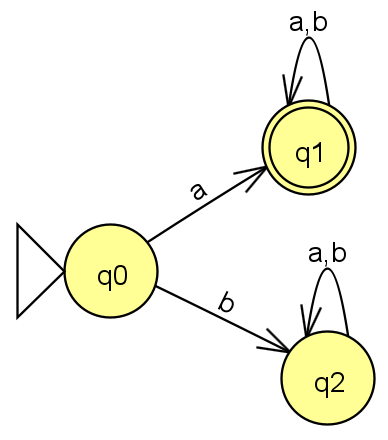
\includegraphics[width=0.2\textwidth]{../../../images/DFAs/ex1_q1.png}
\end{center}

\end{document}
